\documentclass[12pt,a4paper]{article}
\usepackage[utf8]{inputenc}
\usepackage[english]{babel}
\usepackage{amsmath}
\usepackage{amsfonts}
\usepackage{amssymb}
\usepackage[left=2cm,right=2cm,top=2cm,bottom=2cm]{geometry}
\author{Adrian Bach}
\title{Using artificial intelligence to improve decision-making in conservation conflicts \\\medskip Ten-week report}

% bibliography 
\usepackage{natbib}
\bibliographystyle{humannat}

\begin{document}
\maketitle

%\newpage
\tableofcontents

\newpage
\section{Conservation}

%6th mass extinction? Ref: \\
At the beginning of what could be a new mass extinction episode (LACKS REF), preserving the remaining "nature" is a central concern for humanity.
Many convictions can justify this statement, but the fact is that we undeniably depend on the services ecosystems provide us. (no need for references, right?)
Pollination, soil enrichment, water treatment, carbon dioxide fixation, among many more, are essential for human survival (REF) and the role of nature in human well-being is increasingly recognized (REF).
However, the key for the permanence of ecosystems is diversity, as it ensures a quick and dynamic response to change(REF).
Note that this variety is often an inspiration for innovation in any kind of technology.
Thus, conservation of biodiversity have become a leading field in ecology.
%
%One of the many aspects, intense competition/antagonism between human activity and wildlife. Ref: \\
%Conservation as a way to tame this problem. Ref: \\
%
%\subsection{Conservation}

According to ... Definition of conservation.
%Different kinds of conservation actions.
Conservation can be applied in many different ways.
It can be preventive, by establishing protected areas to preserve intact ecosystems from human impact \citep{vanwilgen2011critical, bainbridge2017goose}, or to restore already damage ecosystems \citep{rumpff2011state}. 
%: protection areas, ?. Ref: Wilgen2011, Brainbridge2017.
It can also be in reaction to a ongoing problem without preventing contact, \textit{e.g.} culling control by monetary incentives \citep{mason2017changing, cusack2018time}.
Another example is offsetting, which is implementing elsewhere the natural features damaged somewhere by human activity \citep{gordon2011assessing}.
%But conserving a species for its own sakes sometimes lead it to reach numbers being problematic for human activities. Ref: Redpath's book.
There are many other examples, but genuinely successful implementation of conservation is scarce because of the numerous challenges it faces \citep{keith2011uncertainty, vanwilgen2011critical}.

\subsection{Problems faced}

%\subsubsection{Complexity}
Conservation problems are recognized as highly complex and densely interconnected systems, including ecology, sociology, agronomy and climatology simultaneously.
Indeed, socio-ecosystems exhibit most of the characteristics \cite{game2013conservation} attributes to a complex systems: "numerous interacting elements lacking any central control, non-linear interactions between elements, constant change which is seldom reversible, and no clearly defined boundaries".
But, in such systems, it is often impossible to isolate a causes of changes in the system.
%It makes their complete understanding out of our cognition.
%Ref: grimm1999individual, wilgen2011critical, runge2011uncertainty, schluter2013new,pretty much every article I've read.

%\subsubsection{Lack of data}
Since the response to a policy is lost in other signals from a myriad of uncontrollable external factors, monitoring the system's response to a policy over time can be very expensive, time demanding, and often irrelevant, as the number of possible variables is too large.
Thus, conservation policies often lack data to account for their effectiveness, or to understand failure \citep{keith2011uncertainty}.
Furthermore, management is based on estimations of populations, which accuracy varies according to the technique \citep{BUNNEFELD2011441}.
%Ref: rumff2011, all of the articles from the 2011 special edition.

%\subsubsection{Rigidity}
Due to its complexity, predicting the system's response to a change in the conservation policy is very challenging.
It can results in reluctance to change, and in the maintain of inadequate conservation policies \citep{keith2011uncertainty, peterson2005conservation}.
%Ref: geese case, apply a simple protection lead to population reaching conflictual numbers.
Broadly speaking, conservation faces uncertainty at many levels.

%Other limits in keith2011uncertainty about politics and self-serving.
Moreover, conservation often takes place in a political context, and can be significantly slowed, even blocked, by indifferent politics or lobbies for interests that would not benefit from conservation policies \citep{keith2011uncertainty}.
Unexpectedly but fortunately, there is little evidence that bigger budgets make conservation easier or more effective \citep{game2013conservation}.

%Conservation had to be carried on despite these potentially discouraging barriers, acting on protection while dealing with them.
So how to conduct efficient conservation, while dealing with these discouraging barriers and embracing uncertainty?

\section{Adaptive management}
%
%\subsection{Purpose}

%how it deals with certain problems. Acting while acquiring informations, learning from mistakes, closer to the system response to act as quickly as possible.
Adaptive Management (AM) suggests to dynamically update the management policy according to the system's behaviour.
This way, conservation can be better fitted to the system, and acting regularly allow to acquire informations on its response to change.
Therefore, managers can learn heuristically from the system, and react effectively.
%Uncertainty is an irreducible aspect of conservation, so it seems more relevant to act embracing it rather than waiting and keep on with an inadequate policy.
And although AM also relies on the monitoring of some selected variables, their choice can adapt dynamically to the problems detected after each policy updating.
LACKS REF

\subsection{Limits}

%critics from game2013.\\
Yet, \cite{game2013conservation} argues that implementing any new decision will result in a complex change in the system, and that as soon as it has changed it is not comparable to its previous state any more.
This artefact can be reduced in small-scale, simpler systems, to which AM would then be particularly adapted.
%
%other unresolved problems from above.
Even if AM represent one of the most efficient way deals with uncertainty in conservation, it does not include any way to deal with politic-related oppostion.

A major concern in current conservation is that even if a policy effectively protects a species from going extinct, mismanagement can lead populations to reach problematical numbers for human livelihood.

\section{Conflicts}

This is when conflicts arise, because people impacted by a protected population's growth are very likely to defect conservation policies, which can be threatening for the species persistence.
Definition of a conflict. Ref: Redpath's book.\\
ConFooBio is a gathering of well monitored cases of conservation conflicts (see figure \ref{confoobio}).
There are some more examples in (Redpath's book, redpath2013) with leopards etc. YET TO FILL
%mason2017.
and in \cite{behr2017} with wolves and livestock in the french Alps, and Rhinos conservation and illegal poaching for Ivory in south Africa \citep{glynatsi2018evolutionary}.
%Resolving these conflicts requires effective management strategies.
%Management strategy: a sequence of actions on the system in order to achieve goals.\\
%Yet, ecosystems dynamics are highly complex and interconnected, their evolution very difficult to anticipate.

%\subsection{Divergent interests between stakeholders}
In these conflicts, the divergence of stakeholders interests makes conservation even more complicated.
Yet, meeting every stakeholder interests is the only way for a management policy to be sustainable, because defection is less likely.
Indeed, farmers are usually way more interested in the yield they live on, then in the survival of the species that is part of its decreasing.
Reaching a consensus on a target for the population can therefore be an unproductive process.
Moreover, it can prevent the situation from changing in a more equitable way \citep{peterson2005conservation}.

\subsection{MSE}

Management Strategy Evaluation is a framework that describes the process of Adaptive Management in conflictual situations.
It decomposes the problem in four main parts: manager's policy updating, user's harvest strategy, the species population and the mode of estimation of the population (see figure \ref{msediagram}). ADD FIGURE
This structure isolates uncertainty at four main levels: decision-making under uncertainty, the reaction of the users, the population's response,
%links between components of the ecosystems,
and its estimation.
%politics
%All the problems it deals with.
The circular structure is adapted to the heuristic updating of management policy.
Putting manager and user into different parts allow for goal-oriented behaviour.
Unlike consensus-based policies, it recognizes different interests and expectations for conservation,.
It was successfully implemented in fisheries at first, and than applied on terrestrial animals conservation \citep{BUNNEFELD2011441, bunnefeld2013incentivizing}.
%Still need to establish targets.

\section{Modelling}

Since an accurate prediction of these socio-ecosystems' response is hardly possible, any conservation frameworks benefits from a modelling approach.
Conceptual models allow for the rapid exploration of different scenarios under certain hypotheses, thus being very useful decision-helping tools.
%
%\subsection{Different models used in literature}

%Ref: schluter2012, rumpff2011 (dealt with uncertainty by implementing different scenarios), bainbridge2017.
For example, \cite{rumpff2011state} used a Bayesian network to model the transitions between the possible state of a landscape according to a policy, to plan for the restoration of different protected areas previously damaged by human activity.
The book from \cite{schluter2012new} threw the stones of socio-ecological modelling in order to manage conservation involving human compliance (an extensive list of studies using modelling in conservation is presented in chapter 2.1).
In its conclusion, the authors stated that a proper modelling framework for conservation conflicts needs human decision-making modelling, because unforeseen non-compliance was one of the main causes for failures.
The high diversity of models also highlights the lack of common framework, to which MSE is a strong candidate.

\section{Decision-making modelling}

Game Theory (GT), introduced by John Von Neumann and Oskar Morgenstern in 1944 in the book "The Theory of Games and Economic Behavior", is commonly recognized as the leading framework for decision-making modelling.

\subsection{Game theory}
\cite{myerson1997game} describes it as follows: "\textit{the study of mathematical models of conflict and cooperation between intelligent rational decision makers [which choices] affect one another welfare}".
\textit{Games} are simplified vision of actual conflicts, their actual complexity being unreachable.
But such complexity would prevent us from understanding the fundamental issues of conflict and cooperation.
As any other scientific work, game models deliberately omit less relevant details of actual situation to allow the study of particular phenomenon in the scope of a particular question.
In these games, players act in order to maximise the expected value of the game's outcome, the so-called \textit{utility}.
Utility is not necessarily quantified as monetary pay-off, it can be seen in many different ways (time, effort saved, well-being, happiness, ..) and even a mix of them.
Game theoretical perspective can provide insights about: "the strategies different stakeholders will likely adopt given their objectives, [\dots] the range of possible outcomes, [\dots] and whether an optimal or satisfactory solution for all stakeholders can be reached simultaneously" \citep{COLYVAN20111246}.
It was first used in Biology in \cite{maynard1973logic} to investigate the evolution of animal strategies in con-specific fights.
%Definition of the key concepts like utility. Ref: myerson1997.

\subsection{Application to conservation conflicts}
\cite{COLYVAN20111246} investigated theoretical applications of the four main types of games (simple, chicken, stag and prisoner games) to Adaptive Management, but its actual implementation for conservation purposes is fairly novel. 
\cite{glynatsi2018evolutionary} modelled the existing conflict between rhinos protection and illegal poaching for ivory as a common-pool resource problem, to assess which proportion of rhinos should be de-horned to minimize their killing, according to poacher being unconditional or selective killers.\\ %(figure \ref{rhino-poachers-game}).
%\begin{figure}
%	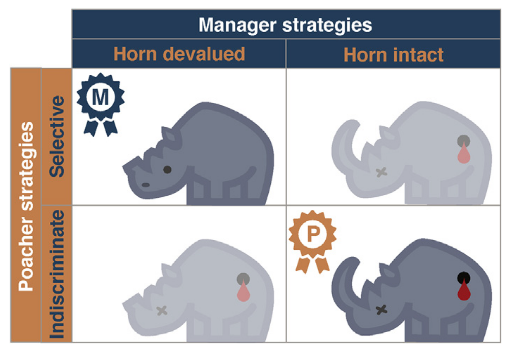
\includegraphics[scale=0.5]{rhinos-poachers-game.png}
%	\caption{The game between rhino manager and rhino poachers. The system settles to one of two equilibriums, either devaluing is eff ective or not. N.E. Glynatsi et al.}
%\end{figure}
Recently, \cite{duthie2018} introduced  a model developed on MSE framework, that includes decision-making modelling within Game Theory.

\section{GMSE} Ref: duthie2018gmse. emphasize on its novelty.

\subsection{Formalisation of MSE framework}

%describe how it falls in MSE framework, how it deals with uncertainty at each level, consensus biases, long term foreseeing.
%At four main levels: population dynamics, links between components of the ecosystems, type of estimation of the population, making the right decision without knowing precisely the outcomes, reaction of the users, politics, response of the system, ...\\
%Explain clearly what it is meant for.
GMSE is a mathematical formalisation of MSE framework, assigning each part a conceptual model.\\
The population changes at each time step according to a spatially explicit, individual-based population dynamic model.\\
Each individual is born, moves, and dies according to probabilities drawn in defined laws to account for the uncertainty on population dynamics.
The population is monitored according to different definable techniques, some of which includes probabilities of detection, thus accounting for the uncertainty about the accuracy of monitoring.\\
The manager model can be parametrized to reflect its conservation goals.
It uses the information from the monitoring to set a policy.
A policy is a set of possible actions associated with a cost for its performance.
The manager has a given budget, and implementing a policy has a cost for him/her.\\
The user model can be parametrized to reflect its aims concerning the population.
There can be several users, and they are modelled independently.
He/she has a given budget, and acts according to the number of actions he/she can perform according to their cost set by the manager, in order to achieve his/her goal.
%\subsection{First IBM in conservation}
%
%"Individualbased
%models (IBMs; also known as agent-based models) are
%used to model the behaviour of a system at an individual level
%by specifying simple rules for agents and allowing them to
%interact. These models allow for complex behaviour to emerge
%from simple interactions, though this comes at some cost to
%interpretation and analysis." Ref: hamblin2012parctical.

\subsection{Decision-making artificial intelligence}

Genetic algorithm. Very accessible worded explanation. ref: hamblin2012practical\\
How is it suited to human decision-making?\\
Also used in solving game theoretical problems. Ref: Maynard Smith 1982.\\\
An example of interaction between IBM and genetic algorithm was in hamblin2009, where the parameter governing the interaction rules in foraging ants where allowed to evolve through a GA.

\subsection{limits}

\subsubsection{Theoretical}

Agents act independently, which is very unlikely. REF???!!\\
Different types of conservation interests.
Would be interesting to implement.\\
Does not consider the do nothing option which is sometimes interesting.\\
Measure of conflict intensity?

\subsubsection{Computational}
Computing time when the number of stakeholders increases.\\
Lacks machine learning to be a proper artificial intelligence.\\
Parallelism in general.

\section{Research Questions}

They have to be very closely related to conservation (to avoid making it a mere modelling project)

\subsection{Case study: Geese}

Description. Ref: mason2017, brainbridge2017.
Its attributes (liked with the limits of GMSE). 

from now on always speak about goose, state and farmers to settle the problem in the context of geese

\subsection{Is waiting an interesting option for managers?}

Recently introduced in iacona2017evolutionary: optimal delay before using funds.

\subsubsection{Calculus of impact}
Dr Ascelin Gordon: the difference in the variable of interest when manager acts or do nothing.\\
Implementing the 'doing nothing' option in GMSE. Quantitatively assess the impact on repeated simulations. Mean deviation from conservation target at each time step.\\
According to duthie2018gmse. The number of extinctions over several simulations increases exponentially with the frequence of manager non-intervention. So, I suspect it is going to show that doing nothing is not sustainable as a policy in itself. Surprise!
But is it necessary to act as each time step, "as soon as possible"?

\subsubsection{Action threshold}
Currently in GMSE, a parameter sets the number of the manager's interventions per time step. Rigid, insensible to the situation, action if pop $>$ ou $<$ target, regardless of the size of this difference. acting even if the population if only a few individuals from the target.\\
First, fixed deviation from manager's target as an action threshold. has to be relative the the population size though, if population size is 100, 50 individuals missing or extra is very concerning, yet it is less if population size is tens of thousands. For example I could test thresholds of 1, 5, 10, \dots \% of target.\\ 
Quantitative assessment of the impact on the "quality" of the policy over repeated simulations for increasing threshold values: mean deviation from manager's target? Impact? Conflict reduction? number of extinctions? (Is there a chance that the result will be the same as the manager intervention frequency?)\\
Dynamic threshold? A function of deviation from target, or conflict intensity, that would modify the action threshold.\\
Waiting could imply saving a certain amount of budget for next step. Something that could also concern the users, maybe highlighting a best time to act.

\subsection{Including human values in adaptive management}

All conservationists have different goals according to their values, it would be interesting to implement this. Using the framework from futureconservation.org, I could use quantitative measures of conservationists values and attribute utilities accordingly, and assess if it indeed produce the expected results. Users yields and population size according to the value on nature - people axis, and to conservation - capitalism one. 

\subsection{Standing alone: how to manage a conservation conflict with interacting users?}

Possibly interaction among users, the information they perceive on their neighbours could influence their strategy.

\section{Expected outputs}

At least a paper on the action threshold, a talk in Newcastle, a poster in winter symposium, a participation at the Trondheim workshop. Updated version of GMSE. Field work for SNH, possibly in the policy team to which Aileen is close.

\newpage
\bibliography{10WRbib}
\nocite{*}

\end{document}